\chapter{Design}
\label{cha:design}

\begin{comment}
Chapter 3: Design
This chapter starts to describe the student's own work. It is where the main design aspects of the project are described. The style of presentation may reflect the life cycle of the project, for example commencing with the Requirements Analysis, but it should not read like a diary. The design should be clearly and precisely described with supporting diagrams. The presentation should be at a fairly high level without excessive detail. This chapter is a suitable place to justify your choice of architecture, implementation technologies and APIs used.
\plan{This section contains my PLAN of what I will do (before I started) of my app, it should be programming language independent}
\end{comment}

This chapter covers design of the system, including an overview of the architecture and descriptions of the key components. 

\section{Statement Management}
The statement management features of the application were selected based on the functionality observed during the background research and conversations with potential users, asking what features they enjoyed from their current Internet banking and what additional features they would find useful to manage their statements

The key features include; parsing of files downloaded from Internet banking, mapping transactions found in the files to real world businesses (transactors), organising transaction history by \gls{category} or transactor and viewing all transactions at a particular transactor.

\subsection{Upload} \label{subsection:upload}
To get a users transaction history they must first upload a file containing their historical transactions.

The major UK banks tested\footnote{Natwest, First Direct and HSBC} provided statement downloads in Quicken, Microsoft Money or Microsoft Excel format. Further investigation revealed that the underlying formats were Quicken Interchange Format (QIF), Open Financial Exchange (OFX) and comma-separated values (CSV).

As there is no pre-defined standard for bank statements in CSV format, upon investigation, it became clear that the banks used completely different structures. It was decided the application would parse the QIF and OFX formats, following their respective specifications. Examples of QIF and OFX can be seen in Fig. \ref{fig:qifofxformat}.

It was quickly identified that although the QIF/OFX files were following the same specification, depending on the bank they had different structures, and in some cases the structures even varied from the same bank, depending on the exact wording of the download. Interestingly a OFX file downloaded from First Direct was found to be in QIF format, despite an \lstinline$.ofx$ suffix.

Notably there were discrepancies with the formatting of dates in QIF. The specification from Intuit\footnote{The developers of Quicken and QIF} doesn't specify a date format \cite{quiken2010qif}. The sample files tested included dates in D-M-Y, M-D-Y and Y-M-D format.

\begin{figure}
\centering
\begin{lstlisting}
% QIF FORMAT
!Type:Bank
D28-06-13
PASDA SUPERSTORE    TROWBRIDGE
T-15.00
^
D28-06-13
PPAYPAL PAYMENT
T-12.50
^
\end{lstlisting}
\caption{Two transactions in QIF format}

\begin{lstlisting}
% OFX FORMAT
<STMTTRN>
<TRNTYPE>POS</TRNTYPE>
<DTPOSTED>20130628</DTPOSTED>
<TRNAMT>-15.00</TRNAMT>
<NAME>ASDA SUPERSTORE</NAME>
<MEMO>TROWBRIDGE</MEMO>
</STMTTRN>
<STMTTRN>
<TRNTYPE>DEBIT</TRNTYPE>
<DTPOSTED>20130618</DTPOSTED>
<TRNAMT>-12.50</TRNAMT>
<NAME>PAYPAL PAYMENT</NAME>
</STMTTRN>
\end{lstlisting}
\caption{Two transactions in OFX format}
%\label{QIF compared to OFX for two identical transactions}
\label{fig:qifofxformat}

\end{figure}

To combat this three steps of resiliency were added to the design of the upload system, seen in Fig. \ref{fig:fileupload} \todo{Recompile this figure}.

\begin{figure}[h]
    \centering
    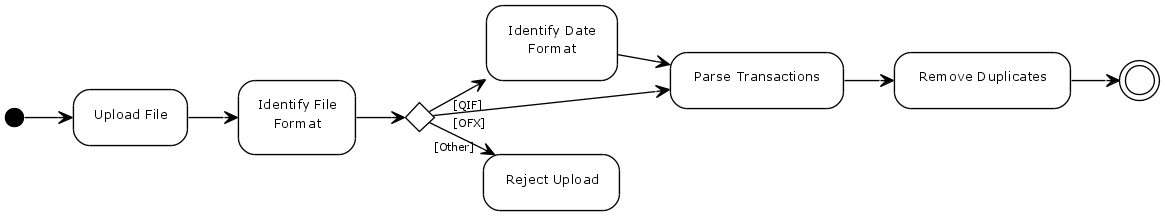
\includegraphics[width=\textwidth]{design/upload-activity}
    \caption{Activity diagram for statement uploads}
    \label{fig:fileupload}
    
    \begin{comment}
(start)->(Upload File)->(Identify File Format)-><a>[QIF]->(Identify Date Format)->(Parse Transactions),
<a>[OFX]->(Parse Transactions)->(Remove Duplicates)->(end),
<a>[Other]->(Reject Upload)
    \end{comment}
\end{figure}

Having uploaded the file the system first identifies the filetype by looking inside the file and parsing its contents, ignoring the extension and rejecting the file if it matches neither format.

If the file is QIF the parser parses all transactions up front and evaluates the format of the dates. If the dates are found to have the format \lstinline$\d00-00-0000$ the system needs to decide whether that's D-M-Y or M-D-Y, otherwise performing standard date parsing of the string.
%(\lstinline$\d{1,2}[/-]\d{1,2}[/-]\d{2,4}$ in regular expression)
%
To decide between D-M-Y or M-D-Y the application goes through all the dates and attempts to parse in both formats, if a format fails it is marked as incorrect. This leaves the application in one of the four states, seen in Table \ref{table:datestates}. In the case of state 1 or 4 there is ambiguity and the application prompts the user. This ambiguity can be caused by dates that are malformed or a collection of dates falling within a range that doesn't have a day value over 12, as both formats parse correctly. 

\begin{table}[h]
\centering
\begin{tabular}{lll}
State & D-M-Y & M-D-Y \\
1     & true  & true  \\
2     & true  & false \\
3     & false & true  \\
4     & false & false
\end{tabular}
\caption{Possible states following evaluation of transaction dates}
\label{table:datestates}
\end{table}

In provisional user testing, it was discovered that users had a tendency to upload the same file more than once or to upload statements with an overlapping date range. To account for this, before creating a new Transaction the application checks for an identical transaction for the current user in the database and if one is found, skips creating a new Transaction. For speed this is done using a stored unique value, resulting from a SHA512 hash of date posted, transaction value, transactor, memo and transaction id\footnote{If a one was provided by the users bank}, which is generated when saving a Transaction to the database.

% 

\subsection{Named Entity Resolution}
Almost all functionality of the project relies on successfully mapping the text found on a bank statement that represents a business or person to a single entity in the application, known as a \gls{transactor} by the system. After a cleanup of different suffixes that banks append it was found that \glspl{transactor} are often referenced using several names.

Seen in Table \ref{tab:sainsburys}, Sainsbury's was referred to nine different ways in the statement data uploaded by the research participants and similar results are found for most \glspl{transactor}.

\begin{table}[h]
\centering
% SELECT name,count(t.id) as count FROM `transaction` AS t LEFT JOIN global_transactor_mapping AS g ON global_transactor_mapping_id = g.id WHERE global_transactor_mapping_id IN(SELECT id FROM global_transactor_mapping WHERE transactor_id = 7) GROUP BY global_transactor_mapping_id ORDER BY count DESC
\begin{tabular}{@{}ll@{}}
\toprule
Reference            & Occurrences \\ \midrule
sainsburys s/mkts    & 46          \\
sainsburys s/mkt     & 9           \\
sainsburys s/mkts cd & 7           \\
js online grocery    & 2           \\
sainsbury s/mkt cd   & 2           \\
sainsburys smkt      & 2           \\
js online grocer     & 1           \\
sainsburys superma   & 1           \\
sainsburys-superma   & 1           \\ \bottomrule
\end{tabular}
\caption{References to the entity `Sainsbury's' found in participant data}
\label{tab:sainsburys}
\end{table}

\subsubsection{Mapping to Entities}
In consideration of this, the concept of mappings was added to the system. A \gls{mapping} is a single \gls{reference} to a transactor, such as `sainsbury s/mkt'. A transactor has multiple mappings. Fig. \ref{fig:mapping} shows this structure.

\begin{figure}[h]
    \centering
    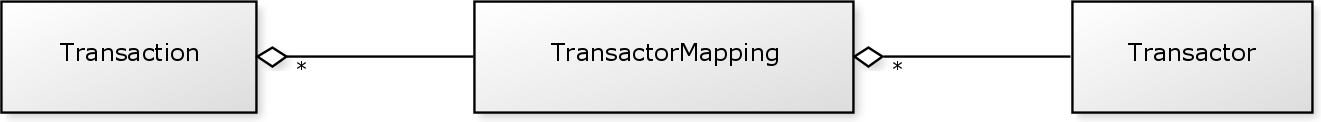
\includegraphics[width=\textwidth]{design/simple-mappings}
    \caption{Overview of Mappings}
    \label{fig:mapping}
    
    \begin{comment}
%[User]-*<>[Transaction]
[Transaction]<>*-[TransactorMapping]
[TransactorMapping]<>*-[Transactor]
    \end{comment}
\end{figure}


\subsubsection{Global vs User}
As identified in the background research, it should be possible for users to both categorise and organise transactions according to their preferences and override existing categories, however categories chosen by a particular user should not affect affect other users. 

To support this the application stores two sets of mappings and transactions, \glslink{usertransactor}{User} and \glslink{globaltransactor}{Global}. The structure of the relevant objects is shown in Fig. \ref{fig:transactormappings}. A Transaction can have both a \glslink{usertransactor}{UserMapping} and a  \glslink{globaltransactor}{GlobalMapping}, in which case the UserMapping overrides the GlobalMapping when calling methods such as \inlinephp{getMapping()} on the Transaction.

\begin{figure}[h]
    \centering
    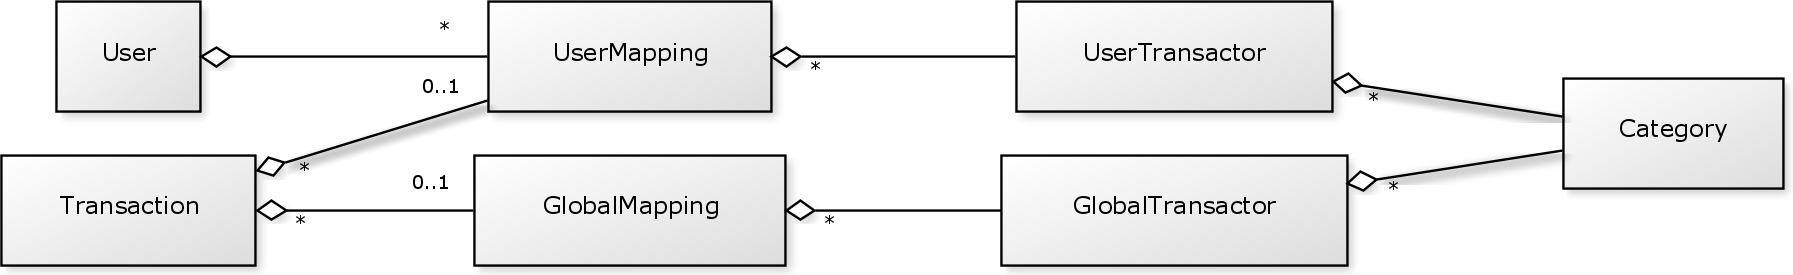
\includegraphics[width=\textwidth]{design/mappings}
    \caption{Overview of User Mappings}
    \label{fig:transactormappings}
    
    \begin{comment}
[Transaction]<>*-0..1[UserMapping]
[Transaction]<>*-0..1-[GlobalMapping]
[User]<>-*[UserMapping]
[UserMapping]<>*-[UserTransactor]
[UserTransactor]<>*-[Category]
[GlobalTransactor]<>*-[Category]
[GlobalMapping]<>*-[GlobalTransactor]
    \end{comment}
\end{figure}

\subsection{Suggestions}
Having mapped \glspl{reference} to entities, the system is able to use this knowledge to make suggestions of appropriate entities for unseen references in some cases to help streamline the naming process for potential users.
%
This is performed by taking the list of mappings and finding those with the smallest difference to the unseen reference. Difference can be calculated in several different ways, including the Levenshtein distance which calculates the number of single-character edits to transform between the two strings, implementation details for this project can be found in Section \ref{section:suggestion-implementation} \cite{levenshtein1966binary}.

\section{Prediction}
In order to make a prediction of how much money a user will spend and receive in a given period two steps need to be completed, predicting whether or not each individual transaction will occur in a given month and estimating how much money will be involved.

Drawing from the research detailed in Chapter \ref{cha:background}, the system uses a First-order Markov Chain model to decide whether or not transactions will occur, and weighted arithmetic means to predict how much money will be spent.

\subsection{Markov Chain Models}
% The probability of a transaction occurring can be calculated using Bayes' Theorem
% Probability of spend given that we didn't spend = probability of not spend given spend * probability of spend over probability of not spend.

An easy way to visualise the Markov Chain Models the system is creating is through a directed graph. Two frequent examples are shown in Fig. \ref{fig:transition-monthly} and \ref{fig:transition-one}, taken from participant data, where $0$ represents a transaction not occurring, $1$ is the opposite and the edges are labelled with the probability of transitioning from one to the other. \todo{Overuse of the word occurring}

\begin{figure}[h]
\centering
\begin{tikzpicture}[start chain=going right]
\node[state, on chain]                 (0) {0};
\node[state, on chain]                 (1) {1};
\
\draw[
    >=latex,
    auto=right,                      % or
    loop above/.style={out=75,in=105,loop},
    every loop,
    ]
     (1) 	edge[loop above]    node {0.86}   (1)
      		edge[bend left]  node {0.14}   (0)
     (0)	edge[loop above]    node {0.8}   (0)
     		edge[bend left=40]  node {0.2}   (1);
\end{tikzpicture}
\caption{Transition diagram for a monthly pay check}
\label{fig:transition-monthly}
\end{figure}

\begin{figure}[h]
\centering
\begin{tikzpicture}[start chain=going right]
\node[state, on chain]                 (0) {0};
\node[state, on chain]                 (1) {1};
\
\draw[
    >=latex,
    auto=right,                      % or
    loop above/.style={out=75,in=105,loop},
    every loop,
    ]
     (1) 	edge[loop above]    node {0}   (1)
      		edge[bend left=40]  node {1}   (0)
     (0)	edge[loop above]    node {0.91}   (0)
     		edge[bend left=40]  node {0.09}   (1);
\end{tikzpicture}
\caption{Transition diagram for a one off purchase}
\label{fig:transition-one}
\end{figure}

\subsection{Weighted Arithmetic Mean}
Having predicted whether a transaction will occur or not the system needs to predict how much money would be spent. A simple way to make this prediction is taking the mean, however initial testing in MatLab revealed that simply taking an average is affected highly by changes in spending patterns and skewed by outliers, in addition a spending pattern that suddenly changes (for example one caused by the user changing supermarket) takes too long to be reflected in the prediction.

Supported by the background research on weighted smoothing, the system uses weighted averages to account for this. A weighted average is similar to an average but each value is scaled in it's effect by a weighting factor, this allows the system to give a higher weight to more recent transactions.

The weighted average calculation used is shown in Fig. \ref{fig:weighting} where $w(t)$ is the weighting function for time $t$, the most recent month is $t = 0$ and $t = n - 1$ is the oldest month. 

\begin{figure}[h]
    \centering
    \[
        \bar{x} = 
        \frac{
                \sum\limits^{n-1}_{t=0}{w(t) \times x_t}
            }{
                \sum\limits_{t=0}^{n-1}{w(t)}
        } 
    \]
    \caption{Weighted arithmetic mean}
    \label{fig:weighting}
\end{figure}

\subsection{Five Model System}
Using weighted averages is part of the story, the system needs to choose appropriate weights for each transaction and the weights chosen will have a different suitability depending on the spending patterns of the user.
% 
During initial research on weighted averages, it was observed that due to the variety of spending patterns caused by users different spending habits, there was not a `one fits all' solution to weighting.
%
For this reason five different weighting functions were selected and when making a prediction the application selects the weighting algorithm most appropriate for the user.

The five weighting functions were selected from a set of eight (shown in Fig. \ref{fig:weightedaveragegraph}) after experimentation with personal finance data in MatLab. They were selected for significant differences in behaviour.
%
There are four main function types: Exponential relationship $w_x = e^{x}$, decay $w_x = {1}/{x + 1}$, power $w_x = x^1 $ and static $w_x = 1$. One exponential, power and static were selected, and two examples of decay with a variable to affecting the speed of the decay. It would be possible to include a scaling parameter (decay constant) for each weighting function, leading to adaptive weights and to use a learning algorithm to select the optimal value for that parameter, this is discussed in Section \ref{section:learningscalingparameter}.

\begin{figure}[h]
    \centering
    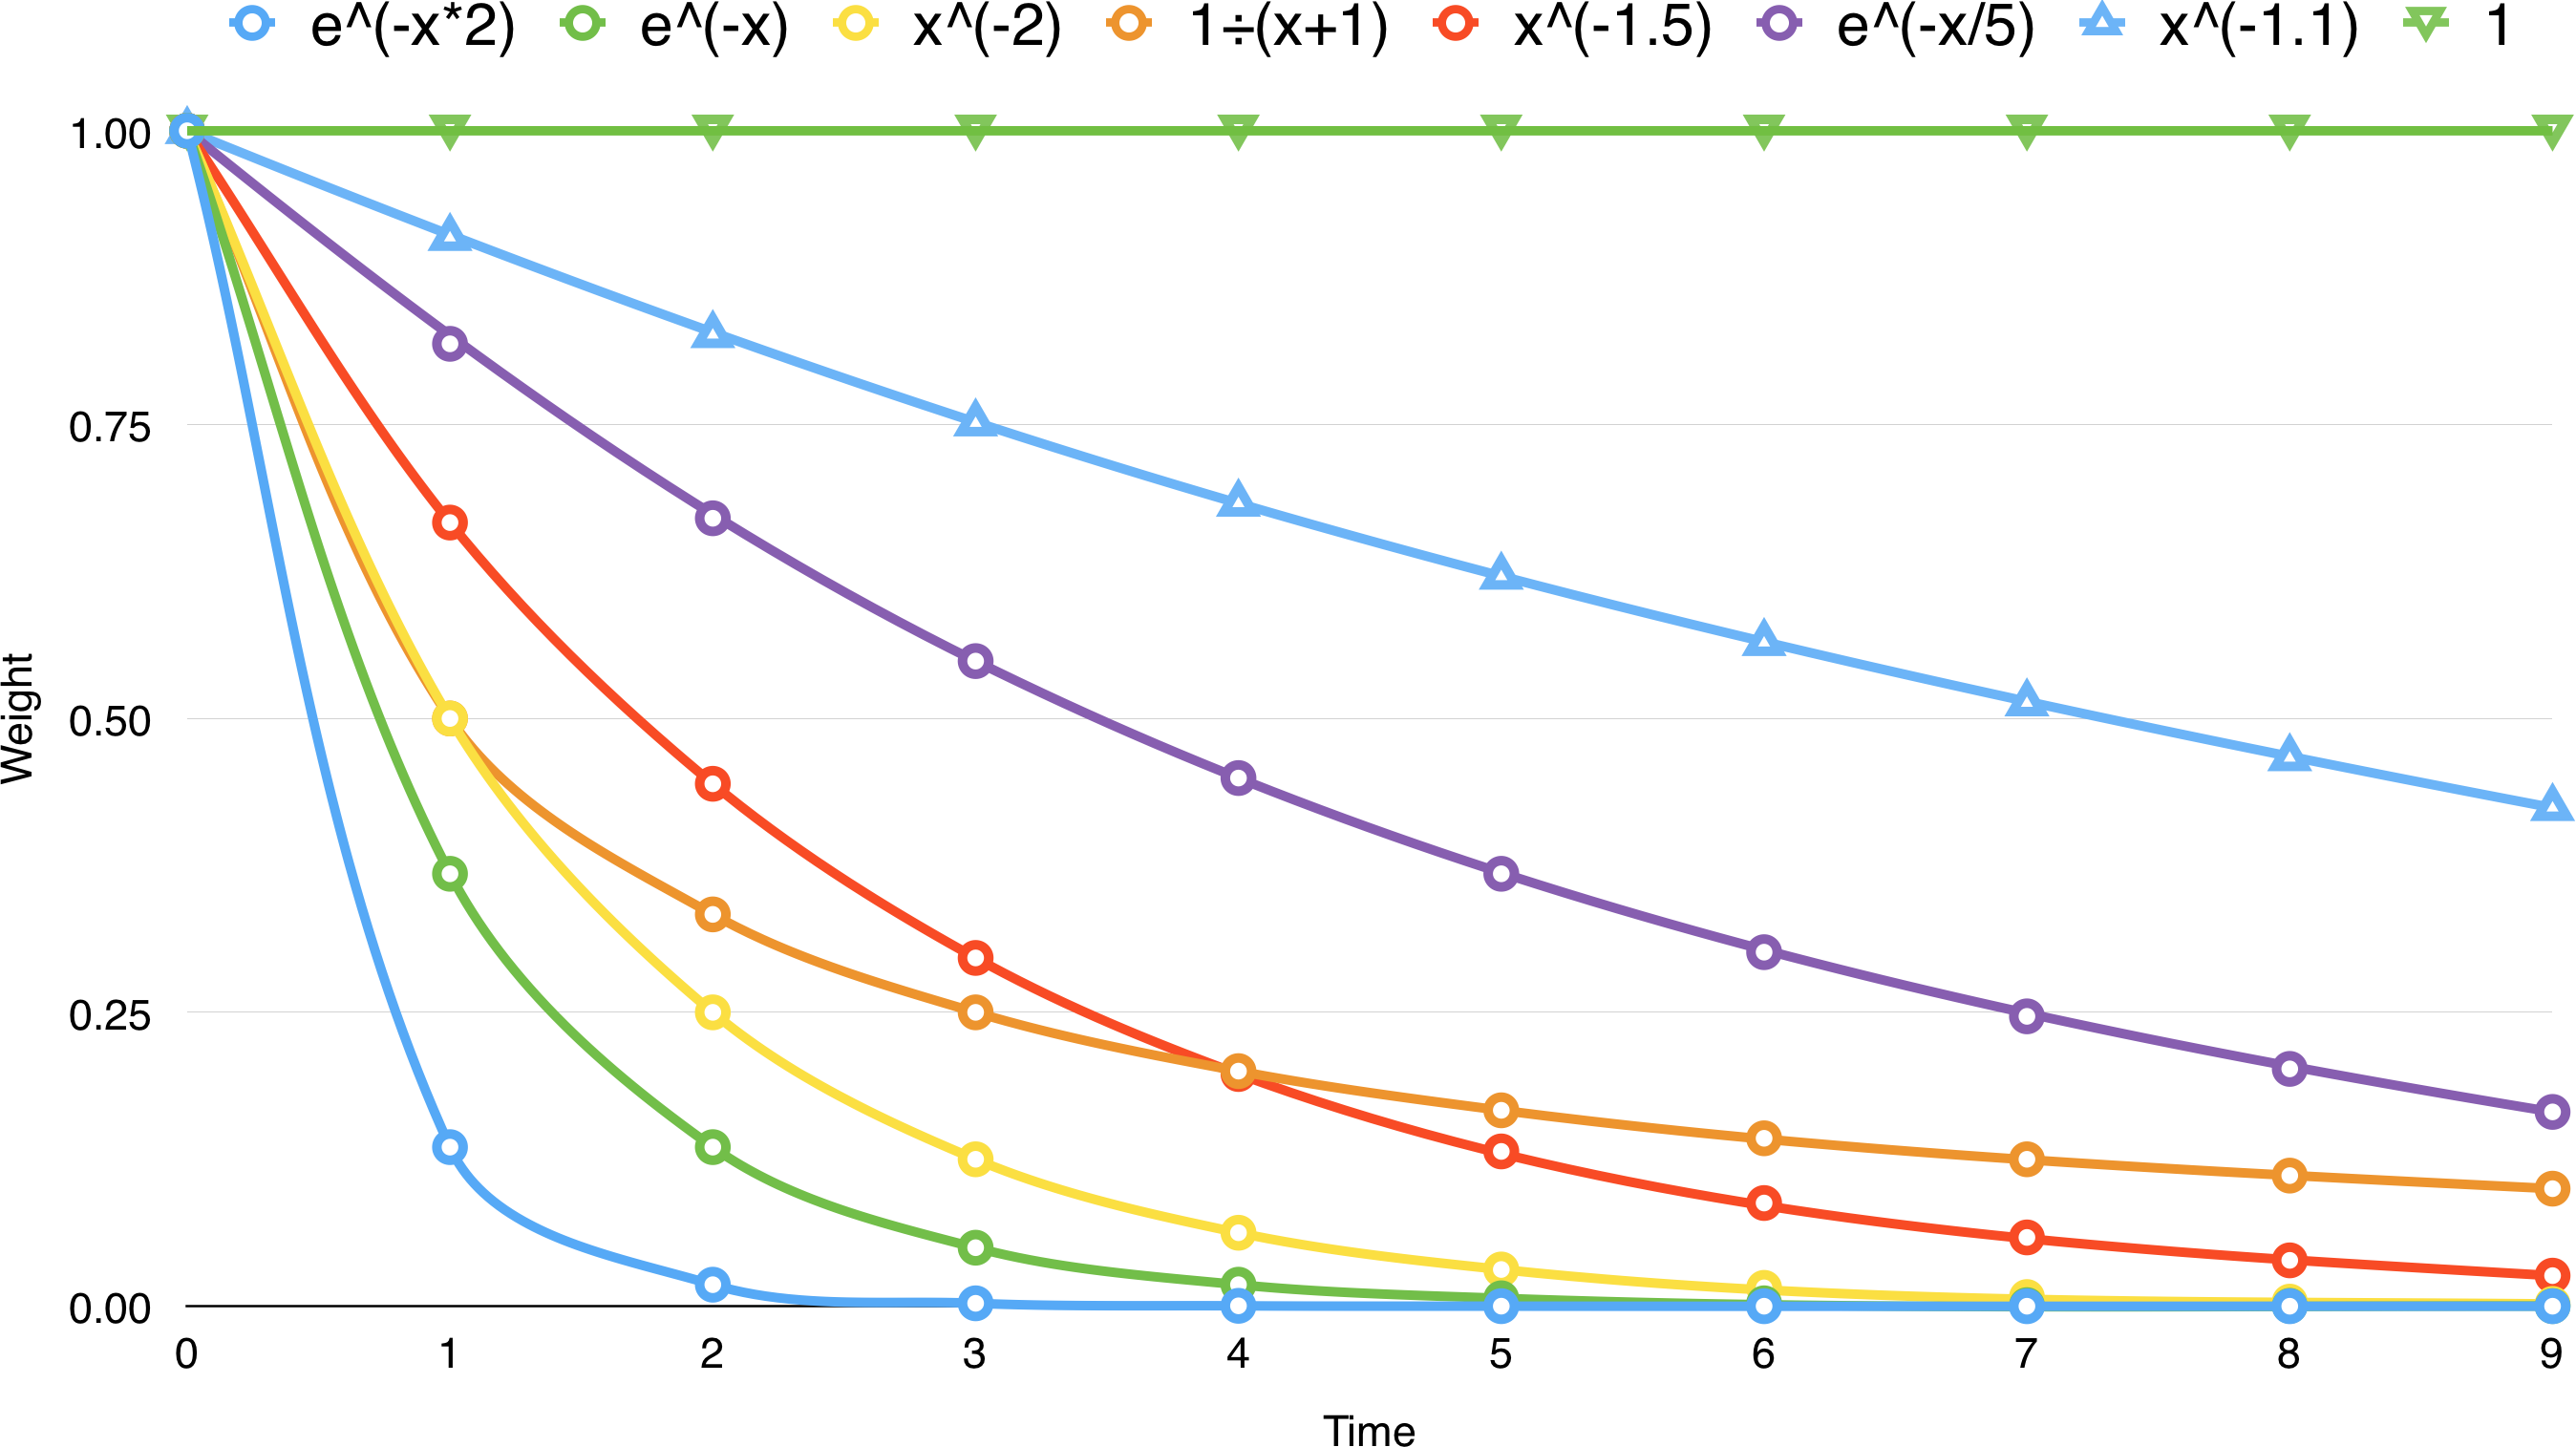
\includegraphics[width=\textwidth]{design/weightedaveragesgraph}
    \caption{The original eight prototype weighting functions}
    \label{fig:weightedaveragegraph}
\end{figure}

To select the best fit weighting function for each user, the system splits the complete months\footnote{Months that have passed fully} from the users transaction history into two parts. Training contains 75\% of months, starting with the oldest and the remaining 25\% (the most recent) is used for testing.
%
If less than four months are available the most recent month is used for testing and the remainder for training. In the case where between zero and two months are available the application falls back on a simple average.

Having split the data the application loops through all the weighting functions available calculating the weighted average of the testing data and evaluating the mean absolute error (Fig. \ref{fig:absoluteerror}) on the training data, by comparing the prediction to the actual value. The function with the least absolute error is best fit to the users overall spending pattern, and so it is selected.

In testing it was discovered that users spending money in similar categories often best suited the same weighting model. Upon further investigation it was discovered that by finding the best weighting model per category in addition to user, on average the absolute error was less. For this reason the most recent implementation of the five model system goes through a users spending in each category, selects the best model for each and uses that to make the prediction in the category. Further research could be done into different levels of modelling and the effect of this level on overfitting, this is discussed in Section \ref{section:overfittingmodels}.

\begin{figure}[h]
    \centering
    \[
        \mathrm{MAE} = \frac{1}{n}\sum_{i=1}^n \left| f_i-y_i\right| 
    \]
    \caption[Mean absolute error formula]{Mean absolute error where $f_i$ is the prediction and $y_i$ is the true value}
    \label{fig:absoluteerror}
\end{figure}

\question{Show how the one with the least error is selected?} \gavin{Yes definately}

\subsection{Confidence}
As the prediction from the Markov Chain Model is based on probabilities it is unstable. To account for this, when making a prediction the application repeats the process of reading from the MCM up to $10,000$ times in one second. The repetition of the reading is used to produce a confidence level of the final prediction once all the results are combined, which is displayed to the user. The confidence level is displayed as a plus/minus value next to the prediction and gives an indication of how sure the application is. 

Assuming the results follow a normal distribution the 95\% confidence interval is calculated by Fig. \ref{fig:confidencelevel} where $\bar{x}$ is the arithmetic mean of the predictions and $x_i$ is the value of prediction $i$.

\begin{figure}[h]
    \centering
    \[
        \bar{x} \pm z \frac{
                        \sqrt{
                            \frac{1}{n}
                            \sum\limits_{i=0}^{n}{(x_i - \bar{x})^2}
                        }
                       }{\sqrt{n}}
    \]
    \caption{Confidence Interval formula}
    \label{fig:confidencelevel}
\end{figure}

\section{Security Considerations}
Strong security is expected of this project, the design considers possible attack vectors and takes steps to prevent or reduce the effectiveness of those attacks.

\subsection{Account Hijacking}
To prevent the security concerns highlighted in section \ref{subsection:account-hijacking} all of the project uses HTTPS, marks cookies as HTTPS only\footnote{Using the Secure attribute}, and redirects users to the HTTPS version if they attempt to access via HTTP. This ensures user data is sent encrypted end to end and cannot be intercepted, preventing access to their authentication details or session cookie.
%
In addition cookies are marked at HttpOnly, ensuring access via non-HTTPS methods such as client side javascript is not possible. This means that even if a users browser is infected with a malicious script for example using XSS (see \ref{subsection:securityother}), the contents of the cookie cannot be read.

\begin{figure}[h]
    \centering
    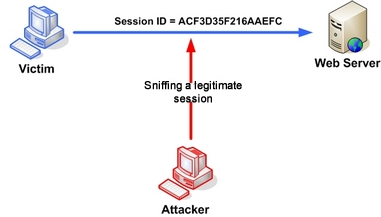
\includegraphics[width=0.70\textwidth]{design/security/sniffing}
    \caption[Obtaining a users cookie using a MitM attack or sniffing]{Obtaining a users cookie using a MitM attack or Sniffing \parencite{owasp2011sessionhihacking}}
    \label{fig:securitysniffing}
\end{figure}

\begin{figure}[h]
    \centering
    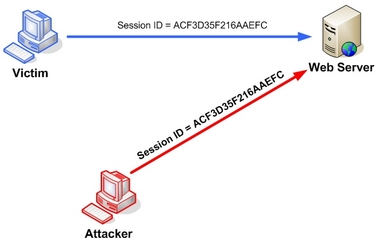
\includegraphics[width=0.70\textwidth]{design/security/hijacking}
    \caption{Performing a session hijack using another users cookie \parencite{owasp2011sessionhihacking}}
    \label{fig:securityhijacking}
\end{figure}

\subsection{Password Security}
 
The project uses Shannon's original equation, calculating the probability of guessing each individual character using a formula that takes into account using a larger character set (such as numbers and symbols) decreases the likely hood of successfully guessing the next character and rejecting a password if it falls below a predefined entropy.
%
Enforcing an entropy threshold rather than enforcing a set of restricting `password rules', was preferred as it gives the user more flexibility hopefully avoiding the annoyance of rules and increases the search space of the passwords. A very long alphanumeric password such as `correct horse battery staple' would be just as valid as a short password containing numbers and symbols such as `6?@7a?Y5R='.

As part of a brute force attack, the attacker may use a dictionary of popular passwords to reduce the testing space before attempting an exhaustion attack.
%
In order to reduce the effectiveness of this kind of attack the project tests any user provided password against a dictionary of at least 50,000 common passwords sourced from password cracking resources \cite{burr2013electronic}.

In addition, to limit the overall effectiveness of brute force attacks, the website rate limits login attempts. If a user attempts to login more than 5 times within one minute, they must wait thirty seconds before they are able to attempt to login again.
%
Rate limiting was chosen over CAPCHA\footnote{Completely Automated Public Turing test to tell Computers and Humans Apart} found on many websites as CAPCHA's slow down users, are often illegible and visual CAPCHA's can prevent visually impaired users from accessing the website \parencite{matt2005inaccessibility, hegarty2012onlinesecurity}. Additionally CAPCHA's can now be solved automatically with a very high success rate using computer vision techniques, and these techniques are already being integrated into brute force software available online \parencite{goodfellow2013neuralnetwork, 9kweu2014captchasolver, danchev2014captcha, savinkin2012captchasolvers}. 

\subsection{Database Storage}
As detailed in section \ref{subsection:databasestorage} security considerations of storing information in a database were considered, the project uses three techniques to help ensure the security of the users information stored in the database. \todo{Broken sentence}

\subsubsection{Passwords}
Passwords are hashed and salted and different hashing functions were investigated. Traditionally functions such as MD5, SHA1 and SHA256 are used to perform the hashing, however due to advances in modern computer equipment it is possible to generate these at an incredibly fast rate, reducing the time taken to brute force a hash.
%
Using a deliberately slow hashing function is designed avoid this problem. Blowfish written by Bruce Schneier is commonly suggested, as it is designed as a computationally expensive operation \parencite{schneier1994description} . This was evaluated with a simple test, calculating as many hashes per possible in one second on the server hosting the project. Table \ref{tab:hashspeed}, shows the results, which found that on average Blowfish took significantly longer to generate each hash\footnote{The code used to perform the test can be found in Appendix \ref{app:hashingtest}}.

For this reason the project salts all passwords and hashes them using Blowfish.

\begin{table}[h]
\begin{tabular}{llll}
         & \multicolumn{3}{l}{Hashes Per Second}                   \\
         & Average & Standard Deviation & 95\% Confidence Interval \\
MD5      & \num{2296667} & \num{12923}  & $\pm 8010$   \\
SHA1     & \num{1869725} & \num{14783}  & $\pm 9162$    \\
BLOWFISH & 17            & 0            & $\pm 0$                 \\
\end{tabular}
\label{tab:hashspeed}
\caption{Average number of hashes completed per second on a 2.7Ghz i7}
\end{table}

\subsubsection{Personally Identifiable Data}
Another concern is personally identifiable data being leaked. In an attempt to avoid this the application encrypts all information stored in the user table, that is needed at a later date using the AES128 encryption standard. This standard was selected for the project as was endorsed by the U.S. National Institute of Standards and Technology, when outlined by NIST in 2001 and has become the ``encryption standard for commercial transactions in the private sector'' \cite{nist2010aes, stair2009informationsystems}.

\subsubsection{Hashing of Usernames}
In addition to the encrypting data needed at a later date the username of each user is hashed so it is only known to the person using that account. In the rare case that any of the passwords were brute forced, the relevant username would also need to be brute forced in order to attempt a login or use the details on another website.

\subsection{Other} \label{subsection:securityother}
Other attack vectors including SQL injection\footnote{A code injection technique that uses maliciously crafted statements to modify the SQL executed} and cross-site scripting\footnote{Inserting client-side scripts to a websites HTML to customise it's logic} (XSS) were also considered.

It was decided that the project would use a prepared statements to reduce the risk of SQL injection. By sending the query followed by the parameters as literal values the database server would not interpret them as an executable portion of SQL and attacks, relying on escaping SQL such as \inlinesql$' OR 1$ are prevented.

In order to mitigate the possibility of XSS the project will need escape all content before displaying it to the user or saving to the database. It was decided that the project would use a templating language that escaped output by default, requiring the output be explicitly marked to avoid escaping.
%
By escaping all content before displaying it to the user a maliciously crafted piece of text such as \inlinehtml$<script>alert(1);</script>$ would be sent to the users browser as \inlinehtml$&lt;script&gt;alert(1);&lt;/script&gt;$ and not interpreted as a script.


\section{Technical Design}
\question{Do I actually need a technical design section? The plan was to include some class diagrams of the project. Leaving this for now.}
\gavin{Yes, some detail, ~2 pages}
\subsection{Object Orientation}
\plan{Patterns used}
\subsection{Domain Class}
\plan{Diagram and list of ALL the objects}
\subsection{UI Design}
\plan{Add photos showing the evolution of the UI}
\subsection{Database Class}
\plan{Diagram of database}
\subsection{External Software and Frameworks}
\plan{What frameworks were used}
\subsection{Platform}
\plan{I decided to use a browser based web application instead of a desktop application}
\subsection{Project Management}
\plan{subsection stuff}
